\section{Zustandsraumdarstellung (ZRD)\formelbuch{265}}
Darstellung einer Differentialgleichung $n$. Ordnung durch ein
Differentialgleichungssystem von $n$ Gleichungen 1. Ordnung.

\subsection{Definition \formelbuch{267}}
\begin{multicols}{2}
	\adjustbox{width=\linewidth}{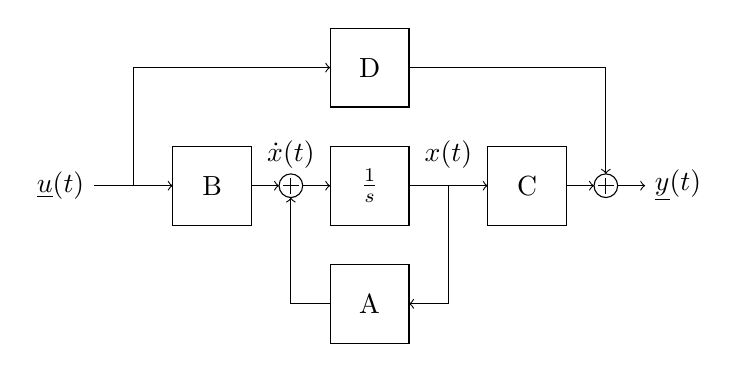
\begin{tikzpicture}
%Names
\node at (0,0) [anchor=east] {$\underline{u}(t)$};
\node at (2.5,0.1) [anchor=south] {$\dot{x}(t)$};
\node at (4.5,0.1) [anchor=south] {$x(t)$};
\node at (7,0) [anchor=west] {$\underline{y}(t)$};

%Boxes
\draw (1,0.5) rectangle (2,-0.5);
\node at (1.5,0) {B};
\draw (3,0.5) rectangle (4,-0.5);
\node at (3.5,0) {$\frac{1}{s}$};
\draw (3,1) rectangle (4,2);
\node at (3.5,1.5) {D};
\draw (3,-1) rectangle (4,-2);
\node at (3.5,-1.5) {A};
\draw (5,0.5) rectangle (6,-0.5);
\node at (5.5,0) {C};

%Operators
\draw (2.5,0) circle (0.15);
\draw (2.4,0) -- (2.6,0);
\draw (2.5,-0.1) -- (2.5,0.1);

\draw (6.5,0) circle (0.15);
\draw (6.4,0) -- (6.6,0);
\draw (6.5,-0.1) -- (6.5,0.1);

%Arrows
%Middle
\draw [->] (0,0) -- (1,0);
\draw [->] (2,0) -- (2.35,0);
\draw [->] (2.65,0) -- (3,0);
\draw [->] (4,0) -- (5,0);
\draw [->] (6,0) -- (6.35,0);
\draw [->] (6.65,0) -- (7,0);
%Top
\draw [->] (0.5,0) -- (0.5,1.5) -- (3,1.5);
\draw [->] (4,1.5) -- (6.5,1.5) -- (6.5,0.15);
%Bottom
\draw [->] (4.5,0) -- (4.5,-1.5) -- (4,-1.5);
\draw [->] (3,-1.5) -- (2.5,-1.5) -- (2.5,-0.15);


\end{tikzpicture}}
	
	Bestimmung der Matrizen A,B,C,D siehe auch \formelbuch{298}
	
	$\dot{\underline{x}}(t) = {\boldsymbol A} \underline{x}(t) + {\boldsymbol B} \underline{u}(t)$ 
  \qquad (Zustandsgleichung) \\
	$\underline{y}(t) = {\boldsymbol C} \underline{x}(t) + {\boldsymbol D} \underline{u}(t)$ \qquad (Ausgangsgleichung)
		
	\begin{description}[noitemsep, style=multiline, leftmargin=15pt]
  		\item[A] Systemmatrix ($n$ x $n$)
  		\item[B] Steuer- oder Eingangsmatrix ($n$ x $m$) ``senkrecht''
  		\item[C] Beobachtungs- oder Ausgangsmatrix ($k$ x $n$) ``waagrecht''
  		\item[D] Übergangs- oder Durchgangsmatrix ($k$ x $m$) \\
  		\item[m] Anzahl Eingänge
  		\item[n] Anzahl Integratoren (Ordnung)
  		\item[k] Anzahl Ausgänge
	\end{description}	
\end{multicols}

\subsection{Äquivalente ZRD\formelbuch{269}}
  \begin{tabular}{p{6cm}p{6cm}p{6cm}}
    \[\underline{\dot{\xi}}(t) = \underbrace{\mathbf{TAT^{-1}}}_{\hat A}\underline\xi(t) +
    \underbrace{\mathbf{TB}}_{\hat B}\underline u(t) \] &
    
    \[ \underline y(t) = \underbrace{\mathbf{CT^{-1}}}_{\hat C}\underline\xi(t) +
    \underbrace{D}_{\hat D}\underline u(t) \] &
    
    $\mathbf{T}$: Transformationsmatrix mit \newline
    $\mathbf{TT^{-1}=T^{-1}T=I}$ \newline
    Mit der Transformationsmatrix kann man verschiedenste Zustandgrössen und ZRD erhalten,
    die aber alle ein identisches Systemverhalten aufweisen.
  \end{tabular}
  
\subsection{Stabilität der inneren Systemzustände \formelbuch{285}}
  Wenn alle Realteile der Eigenwerte $\lambda$ der Systemmatrix ${\boldsymbol A}$
  negativ sind, ist ein LTI-System asymptotisch stabil, \newline
  $\left | \lambda\boldsymbol{I} - \boldsymbol{A} \right |   =0 \rightarrow \forall~\lambda \quad\Re \{\lambda\}<0$
  jedoch nicht umgekehrt. 

\subsection{ZRD im Zeitbereich \formelbuch{270}}

\subsection{ZRD im Frequenzbereich \formelbuch{274} \matlab{ss2tf}}
  \[ \boldsymbol{H(s)} = \frac{\underline{Y}(s)}{\underline{U}(s)} =
  \boldsymbol{C}\left(s\boldsymbol{I}-\boldsymbol{A}\right)^{-1}\boldsymbol{B}+\boldsymbol{D} \qquad
   (\text{Anfangsbedingungen: } \vec{x(0)} = \vec 0) \]
  \\
  Die Grösse der Matrix $\boldsymbol {H(s)}$ entspricht der Grösse der
  Durchgangsmatrix $\boldsymbol D$. $\boldsymbol{I}$ sei die Einheitsmatrix mit
  Grösse $n$ x $n$. \\
  
  Allgemeine Formel für $m=1$ Eingang, $k=1$ Ausgang, $n=2$ Integratoren:  
  \begin{align*}
    H(s) &= \left[
    \begin{array}{c c}
      C_{11}  & C_{12}\\
    \end{array}
    \right] \cdot \left( \left[
    \begin{array}{cc}
      s & 0\\
      0 & s\\
    \end{array}
    \right] - \left[
    \begin{array}{cc}
      A_{11} & A_{12}\\
      A_{21} & A_{22}\\
    \end{array}
    \right] \right)^{-1} \cdot \left[
    \begin{array}{c}
      B_{11}\\
      B_{21}\\
    \end{array}
    \right ]+ D \\
    &=  \frac{B_{11}C_{11}(s-A_{22}) + B_{11}C_{12}A_{21} + B_{21}C_{11}A_{12} + B_{21}C_{12}(s-A_{11})}
		{(s-A_{22})(s-A_{11}) - A_{12}A_{21}} + D
  \end{align*}

  Ist die Übertragungsfunktion $H_{ba}(s)$ vom \textbf{Eingang b} zum \textbf{Ausgang a} gesucht, so gilt:
  \[
    H_{ba}(s) = \frac{Y_a(s)}{U_b(s)} = C(a,:) \cdot (s \cdot I -A)^{-1} \cdot B(:,b) + D(a,b)
  \]


\subsection{Bestimmung der ZRD aus der UTF\formelbuch{277}}
  \[ \boxed{
  H(s)=\frac{Y(s)}{U(s)}=\frac{b_{m} s^{m} + b_{m-1} s^{m-1} +\cdots+b_{1} s 
  + b_{0}}{s^{n} + a_{n-1} s^{n-1} + \cdots + a_{1} s + a_{0}}}
  \]\\


\subsubsection{Regelungsnormalform \formelbuch{277}}
  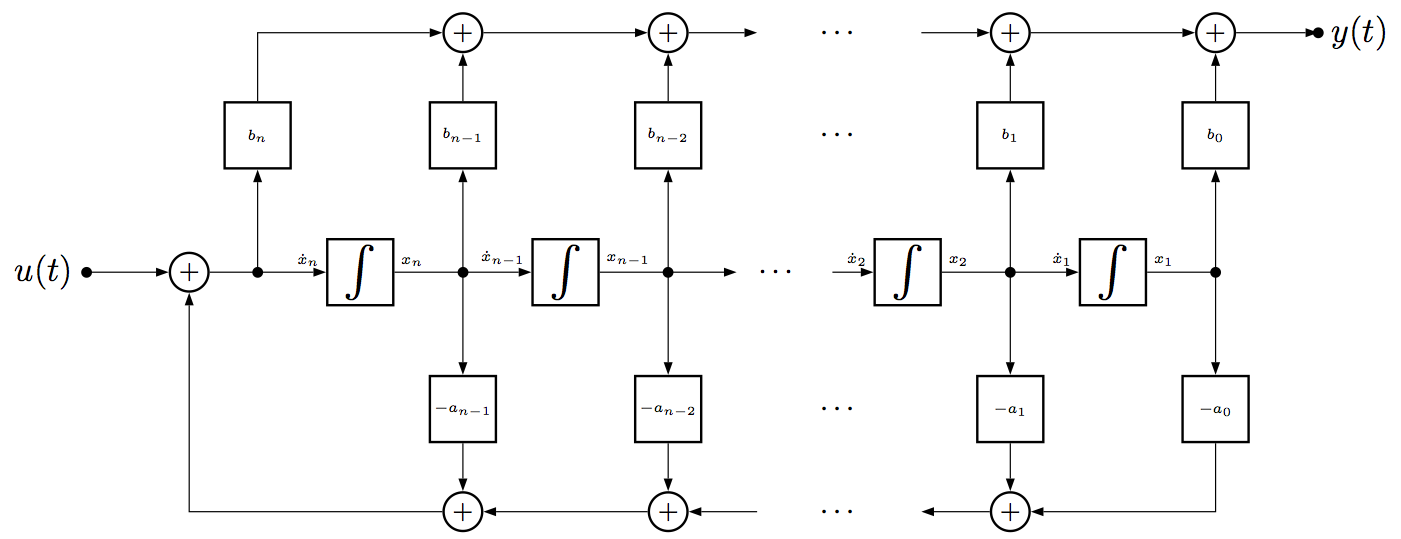
\includegraphics[width=10cm]{./images/zrd-regelungsnormalform.png} \\
  \scriptsize
  \begin{equation*}
    \left [ 
    \begin{array}{c}
      \dot{x}_1(t)\\
      \dot{x}_2(t)\\
      \vdots\\
      \dot{x}_{n-1}(t)\\
      \dot{x}_{n}(t)\\
    \end{array}
    \right ] =
    \left [ 
    \begin{array}{c c c c c}
      0 & 1 & 0 & \ldots & 0\\
      0 & 0 & 1 & \ldots & 0\\
      \vdots & \vdots & \vdots & \ddots & \vdots\\
      0 & 0 & 0 & \ldots & 1\\
      -a_0 & -a_1 & -a_2 & \ldots & -a_{n-1}\\
    \end{array}
    \right ]\cdot
    \left [ 
    \begin{array}{c}
      x_1(t)\\
      x_2(t)\\
      \vdots \\
      x_{n-1}(t)\\
      x_{n}(t)\\
    \end{array}
    \right ]+
    \left [ 
    \begin{array}{c}
      0 \\
      0\\
      \vdots\\
      0\\
      1\\
    \end{array}
    \right ]\cdot
    u(t),
  \end{equation*}
  \begin{equation*}
    y(t) = 
    \left [ 
    \begin{array}{c c c c}
      b_0-a_0b_n & b_1-a_1b_n & \ldots & b_{n-1}-a_{n-1}b_n\\
    \end{array}
    \right ] \cdot
    \left [ 
    \begin{array}{c}
      x_1(t)\\
      x_2(t)\\
      \vdots \\
      x_{n-1}(t)\\
      x_{n}(t)\\
    \end{array}
    \right ]+
    \left [ 
    \begin{array}{c}
      b_n \\
    \end{array}
    \right ] \cdot
    u(t).
  \end{equation*}
  \normalsize

\begin{samepage}
\subsubsection{Beobachtungsnormalform \formelbuch{279 }}
  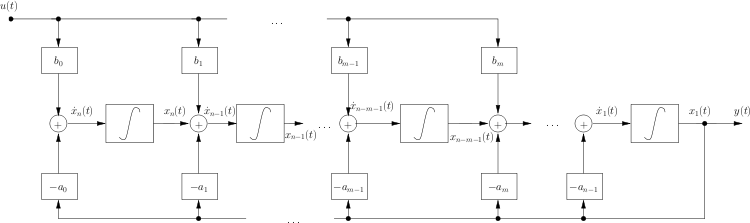
\includegraphics[width=10cm]{./images/zrd-beobachtungsnormalform.png} \\
  \scriptsize
  \begin{eqnarray*}
    \left [ 
    \begin{array}{c}
      \dot{x}_1(t)\\
      \dot{x}_2(t)\\
      \vdots\\
      \dot{x}_{n-1}(t)\\
      \dot{x}_n(t)\\
    \end{array}
    \right ] &=&
    \left [ 
    \begin{array}{c c c c c}
      0 & 0 & 0 & \ldots & -a_0\\
      1 & 0 & 0 & \ldots & -a_1\\
      0 & 1 & 0 & \ldots & -a_2\\
      \vdots & \vdots &  \ddots & 0 & \vdots\\
      0 & 0 & \ldots & 1 & -a_{n-1}\\
    \end{array}
    \right ]\cdot
    \left [ 
    \begin{array}{c}
      x_1(t)\\
      x_2(t)\\
      \vdots \\
      x_{n-1}(t)\\
      x_{n}(t)\\
    \end{array}
    \right ]+
    \left [ 
    \begin{array}{c}
      b_0-a_0b_n \\
      b_1-a_1b_n\\
      b_2-a_2b_n\\
      \vdots\\
      b_{n-1}-a_{n-1}b_n\\
    \end{array}
    \right ]\cdot
    u(t),\\
    y(t) &= &
    \left [ 
    \begin{array}{c c c c}
      0 & 0 & \ldots & 1\\
    \end{array}
    \right ] \cdot
    \left [ 
    \begin{array}{c}
      x_1(t)\\
      x_2(t)\\
      \vdots \\
      x_{n-1}(t)\\
      x_{n}(t)\\
    \end{array}
    \right ]+
    \left [ 
    \begin{array}{c}
      b_n \\
    \end{array}
    \right ] \cdot
    u(t).
  \end{eqnarray*}
  \normalsize
\end{samepage}

%\newpage

\subsubsection{Digaonalform \formelbuch{281}}
\begin{multicols}{2}
  Für einfache, reelle Pole mit $m=n$ \\
  \scriptsize 
    \begin{eqnarray*}
      \begin{bmatrix}
        \dot{x}_1(t) \\
        \dot{x}_2(t) \\
        \vdots \\
        \dot{x}_{n-1}(t) \\
        \dot{x}_n(t)
      \end{bmatrix} &=& \overbrace{ \begin{bmatrix}
        p_1 & 0 & 0 & \ldots & 0 \\
        0 & p_2 & 0 & \ldots & 0 \\
        0 & 0 & p_3 & \ldots & 0 \\
        \vdots & \vdots & \ddots & p_{n-1} & \vdots \\
        0 & 0 & \ldots & 0 & p_n
      \end{bmatrix}}^{\mathbf A} \cdot \begin{bmatrix}
        x_1(t) \\
        x_1(t) \\
        \vdots \\
        x_{n-1}(t) \\
        x_n(t)
      \end{bmatrix} + \overbrace{\begin{bmatrix}
        1 \\
        1 \\
        1 \\
        \vdots \\
        1 \\
      \end{bmatrix}}^{\mathbf{B}} \cdot u(t) \\
      y(t) &=& \overbrace{\begin{bmatrix}
        \alpha_1 & \alpha_2 & \ldots & \alpha_n
      \end{bmatrix}}^{\mathbf{C}} \cdot \begin{bmatrix}
        x_1(t) \\
        x_1(t) \\
        \vdots \\
        x_{n-1}(t) \\
        x_n(t)
      \end{bmatrix} + \overbrace{[b_n]}^{\mathbf{D}} \cdot u(t)
    \end{eqnarray*}
  \normalsize

\columnbreak

  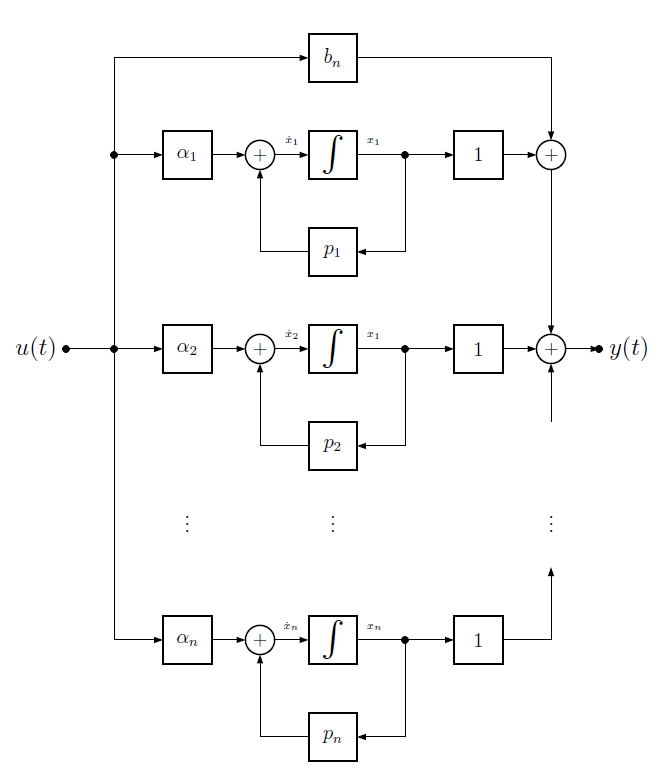
\includegraphics[width=6.5cm]{./images/zrd-diagonalform}
\end{multicols}

\subsubsection{Jordan-Normalform\formelbuch{283}}
  Ist für mehrfache, reelle Pole. Die Jordan-Normalform ist gleich aufgebaut wie die Diagonalform, 
  es kann jedoch auf der oberen Nebendiagonalen z.T 1 haben. 
  Mehr Details im Skript S.283



\subsection{Beobachtbar- \& Steuerbarkeit \formelbuch{287}}
\subsubsection{Steuerbarkeit\formelbuch{287} \matlab{ctrb}}
Gibt es Zustände von $\underline{x} (t)$ die nicht von den
Eingängen $\underline{u} (t)$ beeinflusst werden? Wenn ja,
dann ist das System nicht steuerbar!

Wenn $|Q_{Steuerbarkeit}|= \left| \left [ \boldsymbol{B~~AB~~ A^2B~\ldots~
A^{n-1}B} \right ] \right|  \neq 0$, dann ist das System vollständig steuerbar.

\subsubsection{Ausgangssteuerbarkeit\formelbuch{290}}
Ein System ist vollständig ausgangssteuerbar, wenn es eine Steuerfunktion $\underline{u} (t)$ gibt,
welche die Ausgänge $\underline{y}(t)$ innerhalb einer endlichen Zeitspanne in einen Endwert bringt.

Wenn $rang(Q_{AusgStrbrkeit}) = rang \left( \left [ \boldsymbol{CB~~ CAB~~ CA^2B~\ldots~
CA^{n-1}B ~~ D}\right ] \right) = k$ ($k$= Anzahl Ausgänge), dann ist das System vollständig ausgangssteuerbar. \\
Rang einer Matrix: max. Anzahl lin. unabhängiger Zeilen (= lin. unabh. Spalten)

\subsubsection{Beobachtbarkeit\formelbuch{288} \matlab{obsv}}
Gibt es Zustände $\underline{x}(t)$ die keinen Einfluss auf die Ausgänge
$\underline{y}(t)$ haben? Wenn ja, kann man aus dem Verhalten von 
$\underline{y}(t)$ nicht auf die Zustände $\underline{x}(t)$ schliessen!
Das System ist nicht beobachtbar!


Wenn $|Q_{Beobachtbarkeit}| = \left| \left [ \boldsymbol{
\begin{array}{c}
 C\\
 CA\\
CA^2\\
\vdots \\
CA^{n-1}\\
\end{array}}\right ] \right| \neq 0$, dann ist das System vollständig
beobachtbar.

